\subsubsection{Compito C2: Caricamento di un file in una cartella}

Il compito C2 richiedeva all'utente di creare una nuova cartella denominata "Archivio" all'interno della sezione "Appunti" e di caricare al suo interno il documento "Appunti\_Lezione.pdf" precedentemente posizionato sul desktop. L'obiettivo era valutare l'usabilità dell'interfaccia dedicata all'organizzazione gerarchica e al caricamento dei materiali di studio, con particolare attenzione alla semplicità d'uso dei pulsanti di creazione e all'efficacia della fase di carimento del documento e inserimento dei dati richiesti.

\paragraph{Analisi delle prestazioni generali}

La riprogettazione introdotta nella versione B ha generato un progresso notevole nell'efficacia del compito C2 (Tabella~\ref{tab:6-c2-1}), ferma restando la riuscita del compito per tutti i partecipanti (Success Rate del 100,00\% in entrambe le condizioni). L'aspetto più evidente è la riduzione statisticamente rilevante degli errori medi, ridotti del 75,00\% (da 1,07 a 0,27). Parallelamente, si registra un calo del 48,59\% nel numero medio di click (da 25,93 a 13,33), una variazione sistematica e non attribuibile al caso. Il tempo medio di esecuzione mostra invece una riduzione contenuta che si classifica come una semplice tendenza descrittiva. Sul piano dell'esperienza d'uso, la mediana della difficoltà percepita si attesta stabilmente al valore 2 per entrambe le configurazioni, a indicare che l'attività è stata ritenuta in ogni caso semplice; a livello descrittivo, tuttavia, le medie dei punteggi riportate in figura (2,07 per la versione A e 1,67 per la versione B) delineano una tendenza qualitativa di miglioramento nel livello di sforzo percepito.

\begin{figure}[H]
	\centering
	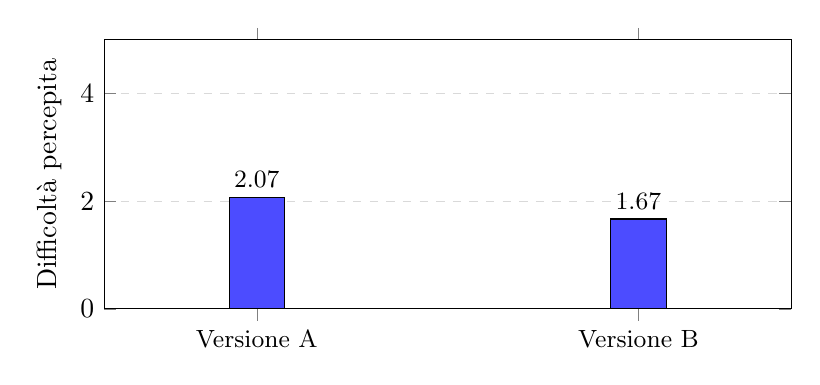
\begin{tikzpicture}
		\begin{axis}[
				ybar,
				bar width=20pt,
				width=0.85\textwidth,
				height=5cm,
				symbolic x coords={Versione A, Versione B},
				xtick=data,
				x tick label style={font=\small},
				ylabel={Difficoltà percepita},
				ymin=0, ymax=5,
				ymajorgrids=true,
				grid style={dashed, gray!30},
				enlarge x limits=0.4,
				nodes near coords,
				every node near coord/.style={font=\small, color=black},
			]
			\addplot+[
				ybar,
				fill=blue!70,
				draw=black
			] coordinates {
					(Versione A,2.07)
					(Versione B,1.67)
				};
		\end{axis}
	\end{tikzpicture}
	\caption{Confronto della difficoltà percepita tra Versione A e Versione B per C2.}
	\label{fig:6-c2-1}
\end{figure}

\begin{table}[H]
	\centering
	\footnotesize
	\renewcommand{\arraystretch}{1.2}
	\caption{Metriche prestazionali globali aggregate per il compito C2.}
	\label{tab:6-c2-1}
	\begin{tabular}{|>{\raggedright\arraybackslash}p{2.2cm}|>{\centering\arraybackslash}p{1.5cm}|>{\centering\arraybackslash}p{1.5cm}|>{\centering\arraybackslash}p{1.5cm}|>{\centering\arraybackslash}p{1.5cm}|>{\centering\arraybackslash}p{1.8cm}|>{\centering\arraybackslash}p{1.6cm}|}
		\hline
		\rowcolor{gray!30}
		\textbf{C2}           & \multicolumn{2}{c|}{\textbf{Versione A}} & \multicolumn{2}{c|}{\textbf{Versione B}} & \textbf{Variazione \%} & \textbf{Rilevanza}                                            \\ \hline
		\textit{Success Rate} & \multicolumn{2}{c|}{100,00\%}            & \multicolumn{2}{c|}{100,00\%}            & \textbf{Invariato}     &                                                               \\ \hline
		\rowcolor{gray!30}
		                      & \textbf{Media}                           & \textbf{DEV.ST}                          & \textbf{Media}         & \textbf{DEV.ST}    & \multicolumn{2}{c|}{}                    \\ \hline
		\textit{Errori}       & 1,07                                     & 1,03280                                  & 0,267                  & 0,45774            & \textbf{-75,00\%}     & \pvalue{0,00856} \\ \hline
		\textit{Tempo}        & 2.13.44                                  & 0,03596                                  & 2.00.08                & 0,01931            & \textbf{-10,17\%}     & \pvalue{0,20212} \\ \hline
		\textit{Click}        & 25,93                                    & 8,85169                                  & 13,33                  & 2,52605            & \textbf{-48,59\%}     & \pvalue{0,00007} \\ \hline
		\rowcolor{gray!30}
		                      & \multicolumn{2}{c|}{\textbf{Mediana}}    & \multicolumn{2}{c|}{\textbf{Mediana}}    & \multicolumn{2}{c|}{}                                                                  \\ \hline
		\textit{Difficoltà}   & \multicolumn{2}{c|}{2}                   & \multicolumn{2}{c|}{2}                   & \multicolumn{2}{c|}{}                                                                  \\ \hline
	\end{tabular}
\end{table}

La drastica diminuzione del numero medio di errori e dei click complessivi testimonia la maggiore linearità introdotta nella versione B. La riorganizzazione dell'interfaccia ha semplificato il processo di caricamento dei file e creazione delle cartelle, riducendo i passaggi superflui senza compromettere la rapidità dell'interazione.

\paragraph{Analisi qualitativa: commenti e osservazioni degli utenti}

I risultati quantitativi trovano riscontro nelle osservazioni raccolte durante le sessioni di test e nei commenti espressi dagli utenti. Per la versione originale (A), sono emerse criticità ricorrenti:

\begin{itemize}
	\item \textbf{Scarsa visibilità dei comandi e layout poco chiaro}: gli utenti hanno riportato difficoltà nell’individuare i controlli per il caricamento dei file e la creazione delle cartelle. Il posizionamento del comando di upload nella parte superiore dell’interfaccia è stato spesso percepito come poco intuitivo.

	\item \textbf{Problemi tecnici e perdita del contesto}: il flusso di caricamento è stato influenzato da un comportamento di refresh della pagina, che ha generato perdita temporanea del contesto operativo. In alcuni casi ciò ha portato alla mancata compilazione di campi obbligatori.

	\item \textbf{Carenze nella validazione e coerenza linguistica}: il sistema non forniva un adeguato supporto nella segnalazione degli errori in caso di campi incompleti. Inoltre, la presenza di etichette in lingua inglese in alcune componenti dell’interfaccia ha ridotto la coerenza linguistica complessiva.
\end{itemize}

Per la versione post-riprogettazione (B), i feedback indicano un miglioramento generale dell’esperienza, con alcune osservazioni residue:

\begin{itemize}
	\item \textbf{Criticità residue nella visibilità delle azioni}: nonostante i significativi miglioramenti riscontrati nelle metriche quantitative, l'operazione ha continuato a generare alcuni dubbi legati al posizionamento dei pulsanti e alla disposizione di determinati elementi dell'interfaccia. Alcuni utenti hanno segnalato come poco intuitiva la posizione iniziale della sidebar dedicata alla navigazione e alla gestione delle cartelle. È stato inoltre suggerito di rendere il pulsante per la creazione di una nuova cartella maggiormente visibile e accessibile, collocandolo in prossimità del pulsante di caricamento dei file. Un'ulteriore osservazione ha riguardato l'etichetta del pulsante utilizzato per il caricamento dei documenti: il termine ``Nuovo'' è stato ritenuto ambiguo poiché associato più facilmente alla creazione di un nuovo elemento (spesso interpretato come una cartella), mentre la dicitura ``Carica'' descriverebbe in modo più chiaro e immediato l'azione effettivamente eseguita.

	\item \textbf{Suggerimenti su flussi operativi alternativi}: è stata segnalata in più casi la mancanza di un flusso ibrido che consenta di caricare un file e creare contestualmente la cartella di destinazione, piuttosto che agire in due momenti separati.
\end{itemize}

\paragraph{Valutazione dell'effetto di apprendimento}

Analizzando i dati in base all'ordine di esecuzione (Tabella~\ref{tab:6-c2-2}), emergono dinamiche estremamente interessanti relative all'apprendimento e all'usabilità delle due interfacce. Nel gruppo che ha affrontato la sequenza A--B, il passaggio alla versione riprogettata si traduce in un miglioramento sistematico e robusto in tutte le metriche. Il tempo medio di completamento scende del 25,02\% (da 2:40.20 a 2:00.13), una contrazione solida e statisticamente rilevante. Registriamo inoltre variazioni sistematiche e non attribuibili al caso sia nella media degli errori, che cala dell'81,82\% (da 1,22 a 0,222), sia nel numero medio di click, ridotto del 48,56\% (da 27,00 a 13,89). Questi risultati indicano che l'esperienza maturata sulla prima interfaccia, unita ai miglioramenti strutturali della seconda, ha ottimizzato notevolmente l'interazione.

Nel gruppo B--A, il quadro si presenta differente. Si osserva un decremento del tempo medio di esecuzione, che tuttavia si qualifica come semplice andamento positivo ma non determinante sotto il profilo inferenziale. Di contro, gli utenti che passano dalla versione B alla versione originale (A) mostrano tendenze di peggioramento nelle altre prestazioni, caratterizzate da un incremento della media degli errori e da un aumento del numero medio di click. Sebbene queste variazioni rappresentino semplici tendenze descrittive (con il numero di click che si avvicina alla soglia di significatività), questo andamento suggerisce che la familiarizzazione con il compito non è bastata a compensare le inefficienze strutturali della vecchia interfaccia A. Gli utenti, pur conoscendo la sequenza di azioni necessarie, sono stati costretti a compiere più errori e click per completare il caricamento del file.

\begin{table}[H]
	\centering
	\footnotesize
	\renewcommand{\arraystretch}{1.2}
	\caption{Confronto delle metriche prestazionali in funzione dell'ordine di esecuzione per il compito C2.}
	\label{tab:6-c2-2}
	\begin{tabular}{|>{\raggedright\arraybackslash}p{2.2cm}|>{\centering\arraybackslash}p{1.0cm}|>{\centering\arraybackslash}p{1.0cm}|>{\centering\arraybackslash}p{1.8cm}|>{\centering\arraybackslash}p{1.6cm}|>{\centering\arraybackslash}p{1.0cm}|>{\centering\arraybackslash}p{1.0cm}|>{\centering\arraybackslash}p{1.8cm}|>{\centering\arraybackslash}p{1.6cm}|}
		\hline
		\rowcolor{gray!30}
		\textbf{Metrica}              & \multicolumn{4}{c|}{\textbf{Ordine A--B}} & \multicolumn{4}{c|}{\textbf{Ordine B--A}}                                                                                                                       \\ \cline{2-9}
		\rowcolor{gray!30}
		                              & \textbf{A}                                & \textbf{B}                                & \textbf{Variazione \%} & \textbf{Rilevanza} & \textbf{B} & \textbf{A} & \textbf{Variazione \%} & \textbf{Rilevanza} \\ \hline
		\textit{Tempo (Media)}        & 2.40.20                                   & 2.00.13                                   & \textbf{-25,02\%}      & \pvalue{0,01312}   & 2.00.00    & 1.33.50    & \textbf{-21,81\%}      & \pvalue{0,09526}   \\ \hline
		\textit{Errori (Media)}       & 1,22                                      & 0,222                                     & \textbf{-81,82\%}      & \pvalue{0,00852}   & 0,333      & 0,83       & \textbf{150,00\%}      & \pvalue{0,29556}   \\ \hline
		\textit{Click (Media)}        & 27,00                                     & 13,89                                     & \textbf{-48,56\%}      & \pvalue{0,00030}   & 12,50      & 24,33      & \textbf{94,67\%}       & \pvalue{0,05806}   \\ \hline
		\textit{Difficoltà (Mediana)} & 1                                         & 1                                         &                        & \pvalue{}          & 2          & 3,5        &                        & \pvalue{}          \\ \hline
	\end{tabular}
\end{table}

Questa asimmetria è confermata e resa visibile dall'analisi della difficoltà percepita (Figura~\ref{fig:6-c2-2}). Nel gruppo con ordine B--A, si rileva un netto incremento della fatica percepita nel passaggio alla vecchia interfaccia: la mediana sale da 2 a 3,5, con un punteggio medio che compie un salto vistoso attestandosi a 3,00 per la Versione A. Questo incremento testimonia come l'abitudine alla fluidità della versione B renda ancora più frustranti le barriere all'usabilità della versione originale. Al contrario, nel gruppo A--B la mediana si attesta a 1 in entrambe le condizioni e i punteggi medi rimangono molto vicini (1,44 per la versione A e 1,56 per la versione B); in questa sequenza, lo sforzo iniziale speso per comprendere l'interfaccia originale sembra aver appiattito la percezione di difficoltà successiva, dove piccoli dettagli della versione B (come l'ambiguità del pulsante ``Nuovo'') hanno bilanciato i benefici strutturali della riprogettazione.

\begin{figure}[H]
	\centering
	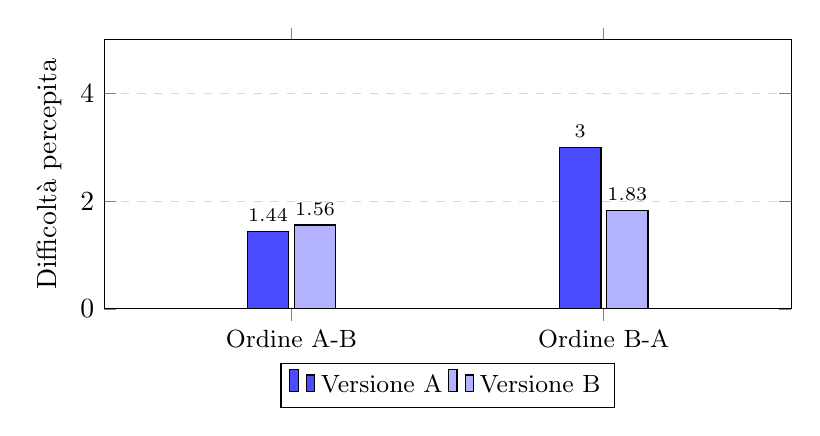
\begin{tikzpicture}
		\begin{axis}[
				ybar,
				bar width=15pt,
				width=0.85\textwidth,
				height=5cm,
				symbolic x coords={Ordine A-B, Ordine B-A},
				xtick=data,
				x tick label style={font=\small},
				ylabel={Difficoltà percepita},
				ymin=0, ymax=5,
				ymajorgrids=true,
				grid style={dashed, gray!30},
				enlarge x limits=0.6,
				legend style={at={(0.5,-0.2)}, anchor=north, legend columns=-1, font=\small},
				nodes near coords,
				every node near coord/.append style={font=\scriptsize, color=black},
			]
			\addplot+[
				fill=blue!70,
				draw=black
			] coordinates {
					(Ordine A-B,1.44)
					(Ordine B-A,3.00)
				};
			\addplot+[
				fill=blue!30,
				draw=black
			] coordinates {
					(Ordine A-B,1.56)
					(Ordine B-A,1.83)
				};
			\legend{Versione A, Versione B}
		\end{axis}
	\end{tikzpicture}
	\caption{Confronto della difficoltà percepita tra Versione A e Versione B per C2 in base all'ordine di esecuzione.}
	\label{fig:6-c2-2}
\end{figure}
